%----------------------------------------------------------------
%
%  File    :  thesis.tex
%
%  Authors :  Keith Andrews, IICM, TU Graz, Austria
%             Manuel Koschuch, FH Campus Wien, Austria
% 
%  Created :  22 Feb 96
% 
%  Changed :  24 March 2009
% 
%----------------------------------------------------------------

% Please send any questions, comments, remarks or complaints to
% manuel.koschuch@fh-campuswien.ac.at


% --- General Setup ---------------------------------------------

%\documentclass[14pt,a4paper,oneside]{extbook} %war 12pt, wieder ändern!!!
\documentclass[12pt,a4paper,oneside]{article} %11original
%\usepackage{times}

%\renewcommand{\rmdefault}{phv} % Arial
%\renewcommand{\sfdefault}{phv} % Arial

\usepackage[utf8]{inputenc}   % so can use Umlaut chars  
\usepackage[T1]{fontenc}
\usepackage[bf,sf]{subfigure}
\renewcommand{\subfigtopskip}{0mm}
\renewcommand{\subfigcapmargin}{0mm}

\usepackage[english]{babel}         % load babel *before* natbi
%\usepackage[austrian]  % load babel *before* natbi
%\usepackage[square]{natbib}                  % citations
\usepackage{enumitem}
\usepackage{url}

\usepackage{float}

\usepackage{latexsym}

\usepackage{color}

\usepackage{ifpdf} % detect outputstyle

\usepackage{geometry} % define pagesize in more detail

\usepackage{fancyhdr} % nicer headers and footers
\usepackage{eurosym}
\usepackage{url}
\usepackage{colortbl} %define colored backgrounds for tables
\usepackage{booktabs}
\usepackage{tabularx}
\usepackage{fancyhdr}
\usepackage{multirow}
\ifpdf
  \usepackage[pdftex]{graphicx}
  \DeclareGraphicsExtensions{.pdf,.jpg,.png}
  \pdfcompresslevel=9
  \pdfpageheight=297mm
  \pdfpagewidth=210mm
\usepackage{fixltx2e}
  \usepackage[         % hyperref should be last package loaded
    pdftex,
    bookmarks,
    bookmarksnumbered,
    linktocpage,
    pagebackref,
    pdfview={Fit},
    pdfstartview={Fit},
    pdfpagemode=UseOutlines,                 % open bookmarks in Acrobat
  ]{hyperref}
  \usepackage{bookmark}
\else                      % latex
  \usepackage{graphicx}
\usepackage[T1]{fontenc} 
{\fontfamily{Schriftart}\selectfont Text}
\usepackage{color}
  \DeclareGraphicsExtensions{.ps}
\fi
 \usepackage{rotating}
\newcommand\tabrotate[1]{\begin{turn}{90}\rlap{#1}\small\end{turn}}

\geometry{a4paper,left=24mm,right=24mm, top=30mm, bottom=30mm} %hier waren original 25,35,30,30

\setlength{\parskip}{3pt plus 1pt minus 0pt}       % vert. space before a paragraph

\setcounter{tocdepth}{1}        % lowest section level entered in ToC
\setcounter{secnumdepth}{2}     % lowest section level still numbered




% --- Start of Document ----------------------------------------


\begin{document}


\begin{picture}(50,50)
\put(-70,40){\hbox{\includegraphics{images/header.png}}}
\end{picture}

\vspace*{-5.8cm}

\begin{center}

\vspace{9.9cm}

\hspace*{-1.0cm} {\LARGE \textbf{Design document\\}}
\vspace{0.2cm}
\hspace*{-1.0cm}  \\

\vspace{0.65cm}


\vspace{0.65cm}
\vspace{3 cm}
\hspace*{-1.0cm} { \textbf{Group Nr. 2\\}}
\vspace{1cm}

\hspace*{-1.0cm} { \textbf{ Lorenzo Haidinger\\}}
\hspace*{-1.0cm} { \textbf{ Ernst Schwaiger\\}}
\hspace*{-1.0cm} { \textbf{ Stefan Ohnewith\\}}
\vspace{0.2cm}
\hspace*{-1.0cm}  \\

\end{center}              % Title Page
\tableofcontents

%--- Include your chapters here ----------

\section{Project description}
\label{chapter1}

The Project description section provides a brief overview of the project, covering the basic idea with simple sketches for visualization.

\subsection{Problem description}

%FIXME: De-uglify diagram (Lorenzo)

The aim of the project is to develop a simplified adaptive cruise control (ACC) system based on two Raspberry Pi 4 devices communicating with each other via Bluetooth. Node 1 is responsible for collecting environmental data using ultrasonic sensors, while Node 2 controls the vehicle speed and interacts with the user via a touch display.

\begin{figure}[h]
	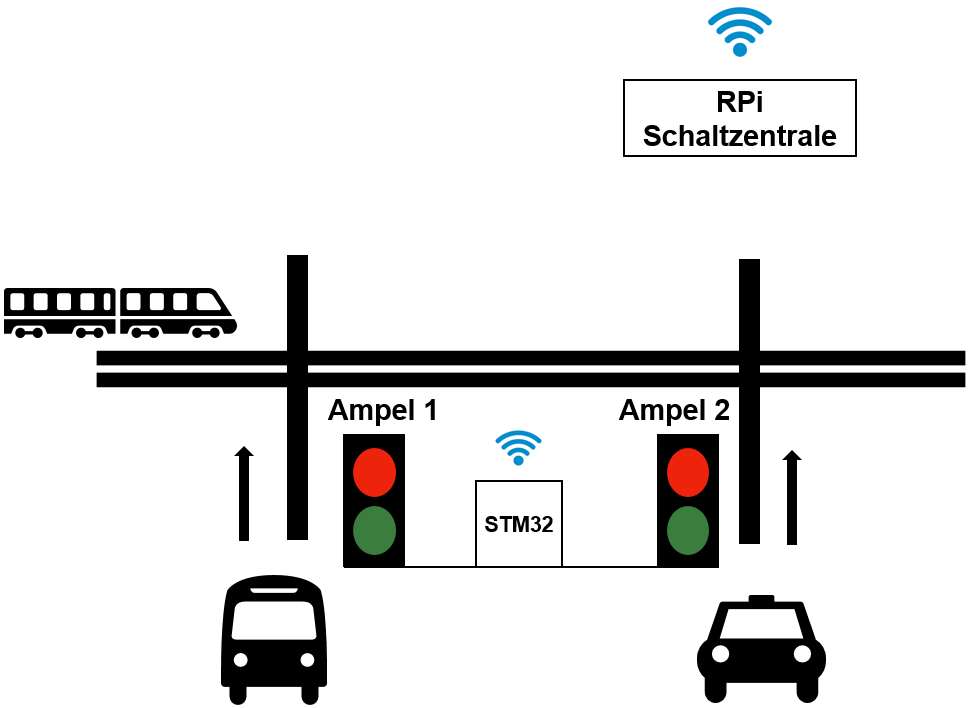
\includegraphics[height=100mm]{images/system}
	\centering
	\caption{system description}
	\label{fig:system}
\end{figure}

\paragraph{}
%The adaptive cruise control (acc) system consists of two nodes, node1, and node2. The nodes are connected by a (FIXME: encrypted/authenticated/both) bluetooth link.

\paragraph{}
Node 1 is equipped with two HC-SR04 ultrasonic sensors that detect cars in front of a virtual vehicle. It performs measurements with both sensors, checks their results for consistency and plausibility, and then transmits the validated values to Node 2. Instead of distance data, the sensor message may also contain error status information which has a different value range than ordinary distance data. The error assumption is that at most one of the two sensors can fail within a defined period of time.

\paragraph{}
Node 2 takes over the function of the steering control unit (ECU) of the virtual vehicle. A control panel on the display can be used to manually increase or decrease the speed of the vehicle, while an additional switch turns the adaptive cruise control (ACC) system on or off. The display shows the current speed and distance values, and the operating status of the ACC (active/inactive/error). Depending on the ACC state, a virtual status display either glows green (active/inactive) or red (error). The requirements for status display, speed and distance displays, and user input can be conveniently implemented using a touchscreen display, for example, with a corresponding \href{https://www.berrybase.at/raspberry-pi-touch-display-2-7-portrait} {Raspberry Pi-compatible device}. 

\paragraph{}
\textbf{Hardware used:}
\begin{itemize}
    \item 2 × Raspberry Pi 4B
    \item 2 × HC-SR04 Ultrasonic Sensor
    \item 1 × Raspberry Pi Touch Display 2, 7" Portrait
\end{itemize}
 
\section{Software architecture and design}
\label{chapter2}

\paragraph
{}
When the ACC is activated, Node 2 executes a periodic task to receive distance measurements from Node 1. Based on these readings, it calculates the updated speed of the virtual car. In case of an alarm situation - such as invalid or missing sensor data, or a loss of Bluetooth communication - the ACC is automatically deactivated and the driver is alerted to take over control.

\subsection{Software modules}

\begin{itemize}
	\item CryptoComm component on Node 1 and Node 2
	\item commThread (Tx) on Node 1
	\item sensorThread on Node 1
	\item commThread (Rx) on Node 2
	\item accThread on Node 2
	\item guiThread on Node 2
\end{itemize}

\subsubsection{Safety related modules}
\begin{enumerate}
	\item sensorThread: \\
		Description: Reads distance measurement from two redundant proximity sensors on Node 1\\
		Functions: (void *)sensorThread(void *)\\
		Data: gCurrentDistanceReading (write)\\
		Requirements see: \ref{req.1}, \ref{req.2} \\
	\item accThread: \\
		Description: Processes received distance readings, turns ACC off and warns in case of an error \\
		Functions: (void *)accThread(void *)\\
		Data: gCurrentDistanceReading (read)\\
		Requirements see: \ref{req.4}, \ref{req.5}, \ref{req.7}, \ref{req.11}, \ref{req.12}, \ref{req.13} \\
	\item guiThread: \\
		Description: Informs the driver about vehicle speed, distance to the next car in front, status of the ACC \\
		Functions: (void *)guiThread(void *)\\
		Data: getter, setter functions shared with accThread \\
		Requirements see: \ref{req.3}, \ref{req.6}, \ref{req.9}, \ref{req.10}, \ref{req.11} \\
	\item commThread (Node 2): \\
		Description: The communication thread on Node 2 receives and validates distance readings, restarts broken Bluetooth connections \\
		Functions: (void *)commThread(void *)\\
		Data: gCurrentDistanceReading (write)\\
		Requirements see: \ref{req.8} \\
\end{enumerate}


\subsubsection{Security related modules}

\begin{enumerate}
	\item CryptoComm: \\
		Description: Session Key generation, MAC generation and validation.; Sending and Receiving Bluetooth.\\
		Functions: TBD\\
		Data: TBD\\
		Requirements see: TBD\\
\end{enumerate}

\subsubsection{Modules with no influence on Safety and Security}

None.

\subsection{Libraries}

Description of used function with parameters.

\begin{enumerate}
	\item LibTomCrypt: \href{https://github.com/libtom/libtomcrypt.git} {https://github.com/libtom/libtomcrypt.git}, used for random number generation, AES session key generation, HMAC generation and verification.
	\item LibTomMath: \href{https://github.com/libtom/libtommath.git} {https://github.com/libtom/libtommath.git}, required by LibTomCrypt.
	\item pigpio: \href{https://github.com/joan2937/pigpio.git} {https://github.com/joan2937/pigpio.git}, used for accessing readings of ultrasonic sensors.
	\item catch2: \href{https://github.com/catchorg/Catch2.git} {https://github.com/catchorg/Catch2.git}, unit test framework
	\item glibc, libstdc++: Posix functions for timestamp retrieval, pthread creation, mutex creation, output stream handling, containers, e.g. std::array
	\item bluez, gio: Libraries for setting up Bluetooth sockets
\end{enumerate}

\subsection{Interrupts}

No interrupts, or interrupt service routines are used in this project.

\subsection{Pinout}

In this subsection, the pinouts are presented separately for Node 1 and Node 2. Since both Nodes are based on a Raspberry Pi, the following diagram \ref{fig:raspi} shows the general pinout configuration of the Raspberry Pi.

\begin{figure}[h]
	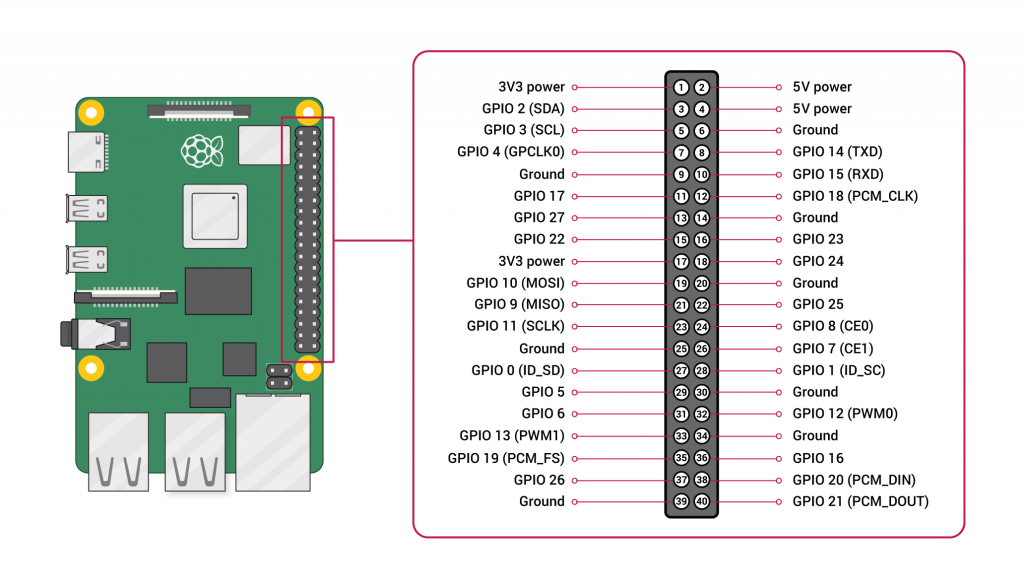
\includegraphics[height=50mm]{images/GPIO-Pinout-Diagram-2.png}
	\centering
	\caption{Raspberry Pi pinout configuration from \href{https://prilchen.de/raspberry-pis-gpio-ein-tor-zu-unzaehligen-projekten/} {prilchen.de}}
	\label{fig:raspi}
\end{figure}

\subsubsection{Node 1}

For Node 1, the ultrasonic sensor (HC-SR04) is connected to the Raspberry Pi. The VCC pin of the sensor is connected to the 5V power pin, while GND is connected to ground. The TRIG pin is wired to GPIO 23, and the ECHO pin is connected to GPIO 24 through a voltage divider using two resistors ($R_1 = 330\,\Omega$ and $R_2 = 470\,\Omega$) to safely reduce the signal from 5V to 3.3V. This can be viewed in Figure \ref{fig:node1-pinout}


\begin{figure}[h]
	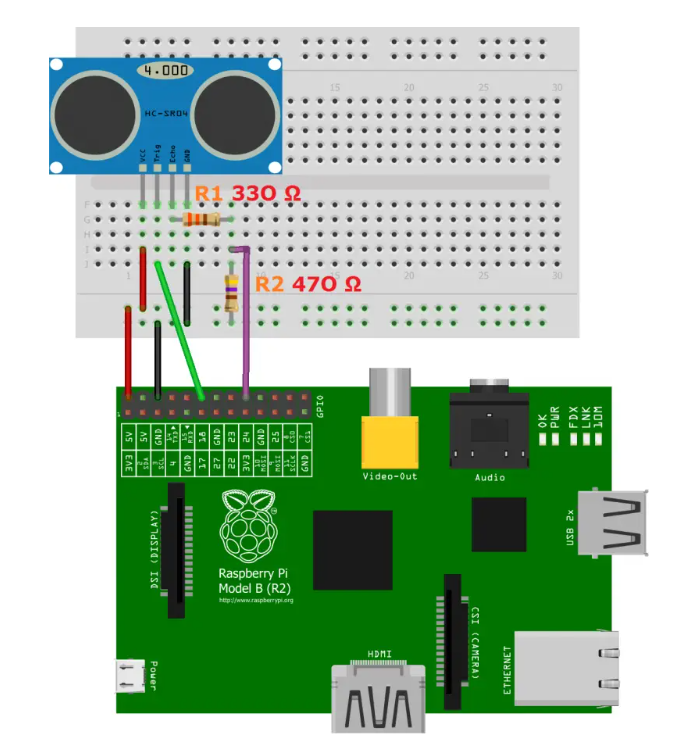
\includegraphics[height=50mm]{images/pinout_node1.png}
	\centering
	\caption{Pinout Node 1}
	\label{fig:node1-pinout}
\end{figure}

\subsubsection{Node 2}

For Node 2, the Raspberry Pi 4 is connected to the Raspberry Pi 7-inch Touch Display.  
The flat DSI ribbon cable is used to transmit the video signal and touch interface, while the four jumper wires provide power and enable I²C communication between the Raspberry Pi and the display controller. The wiring is as follows:

\begin{itemize}
    \item The \textbf{5V pin} of the display (marked ``5V'') is connected to the \textbf{5V power pin} of the Raspberry Pi (pin~4 on the GPIO header) \emph{(red cable)}.
    \item The \textbf{GND pin} of the display (marked ``GND'') is connected to the \textbf{ground pin} of the Raspberry Pi (pin~6 on the GPIO header) \emph{(black cable)}.
    \item The \textbf{SCL pin} of the display is connected to the \textbf{SCL pin} of the Raspberry Pi (pin~5 / GPIO~3) \emph{(yellow cable)}.
    \item The \textbf{SDA pin} of the display is connected to the \textbf{SDA pin} of the Raspberry Pi (pin~3 / GPIO~2) \emph{(green cable)}.
\end{itemize}

The wiring can be seen in Figure \ref{fig:node2-raspy} and \ref{fig:node2-display}.

\begin{figure}[h]
	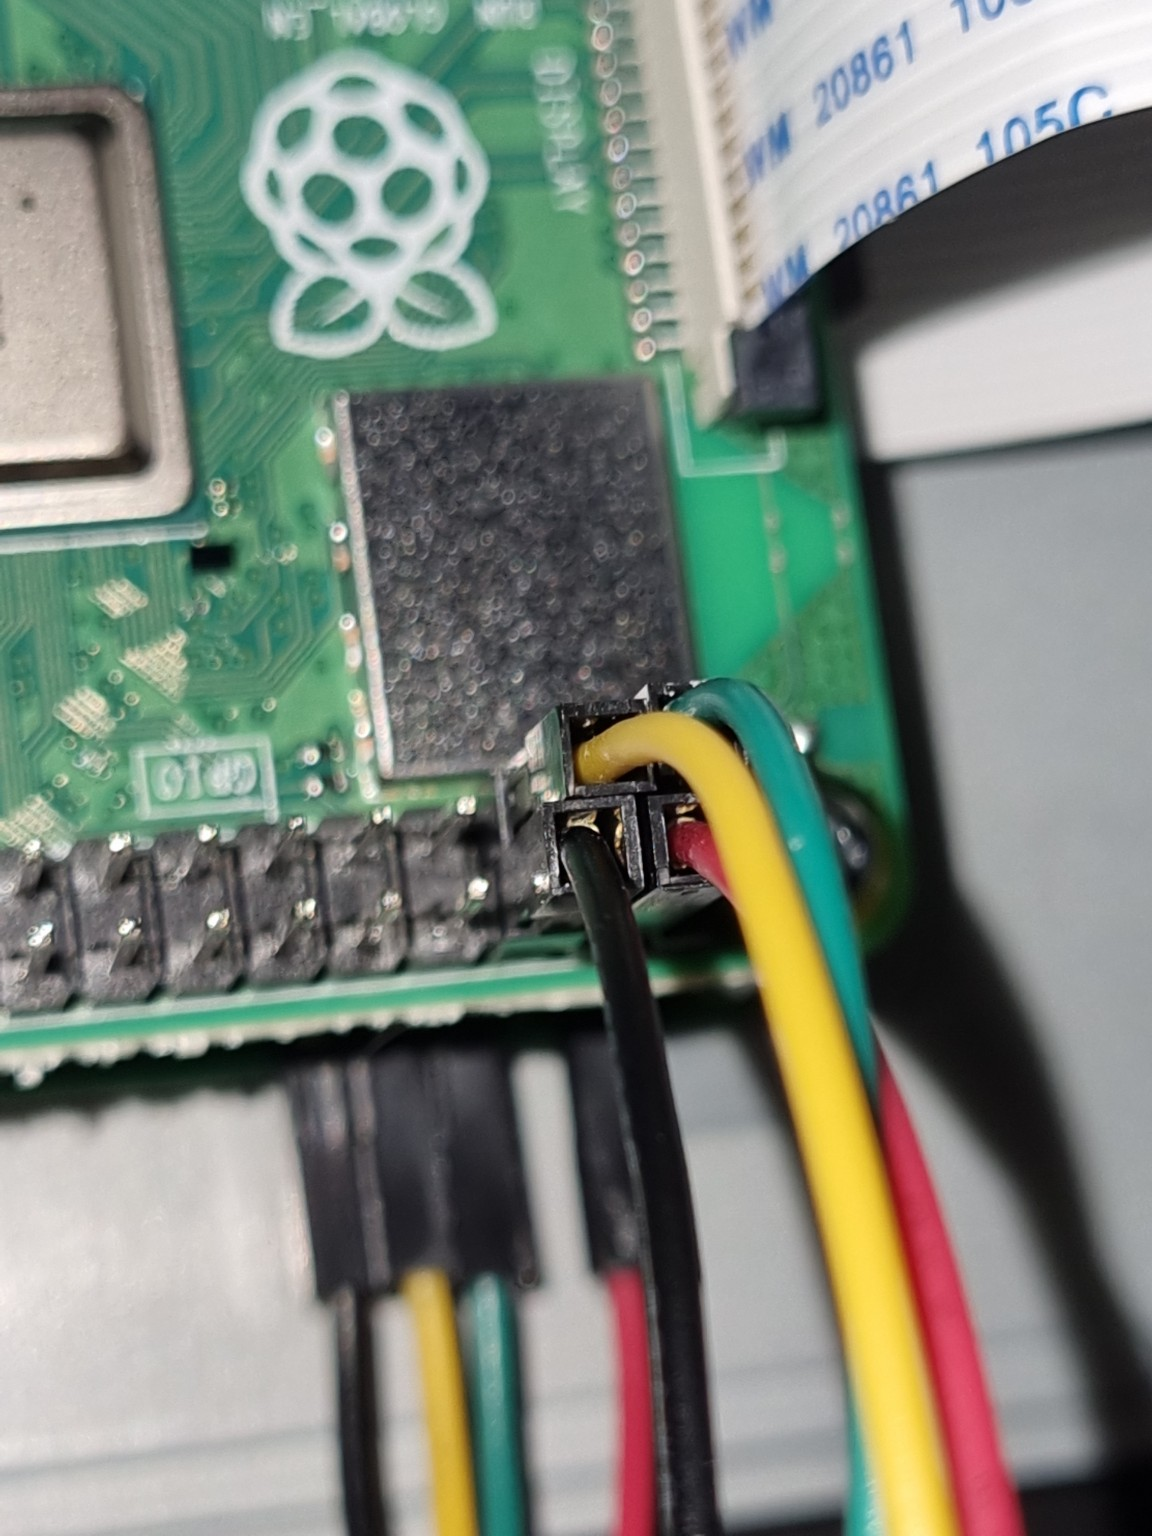
\includegraphics[height=100mm]{images/node2-raspy.jpg}
	\centering
	\caption{Pinout Node 2 Raspberry Pi}
	\label{fig:node2-raspy}
\end{figure}

\begin{figure}[h]
	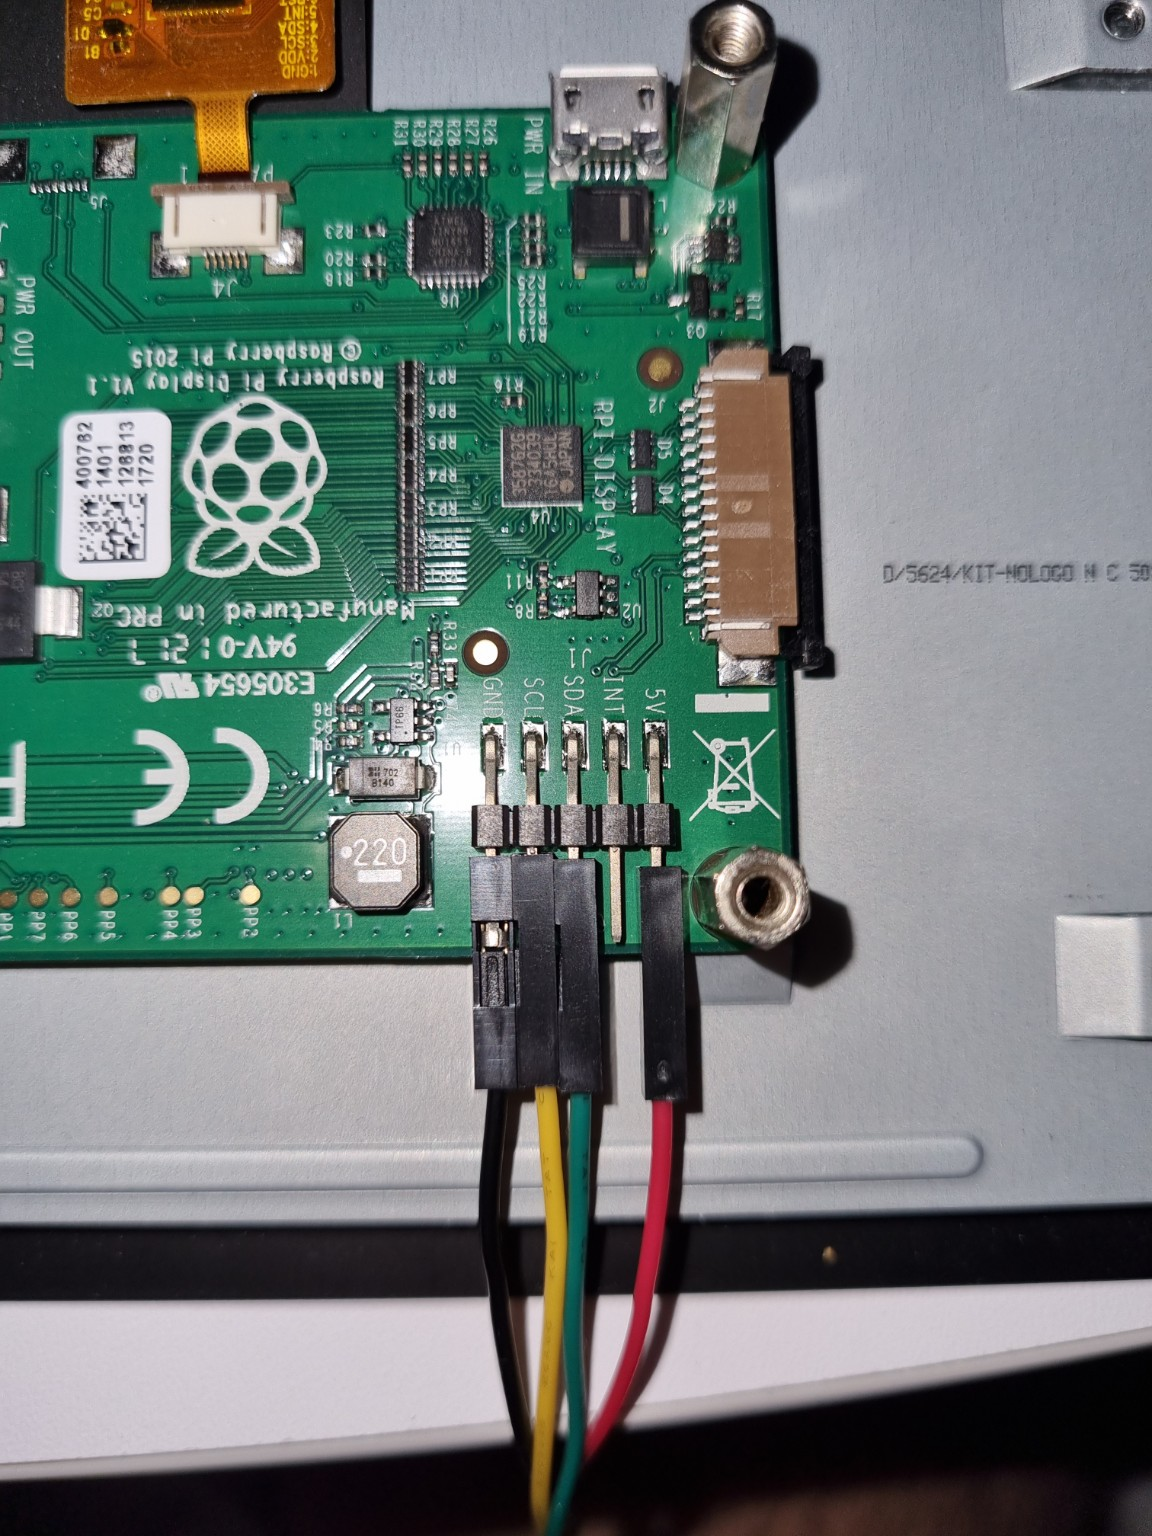
\includegraphics[height=100mm]{images/node2-display.jpg}
	\centering
	\caption{Pinout Node 2 Display}
	\label{fig:node2-display}
\end{figure}

\clearpage
\subsection{GUI}

Figure \ref{fig:gui} shows the dashboard GUI, containing the controls for accelerating and decelerating the vehicle, and for activating adaptive cruise control. It also contains elements showing the vehicles current speed, the distance to the nearest object in front of the car, and the status of the ACC system.

\begin{figure}[h]
	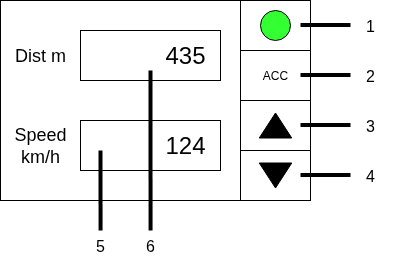
\includegraphics[height=50mm]{images/GUI.png}
	\centering
	\caption{Dashboard GUI}
	\label{fig:gui}
\end{figure}

\begin{enumerate}
  \item ACC Status LED: Shows the status of the ACC system, green if it is in an operational state, red, if ACC  is in a failed state.
  \item ACC Button: Push Button to activate ACC. Can only be pushed if ACC is in operational state.
  \item Accelerate Button: Increases the vehicle speed by 5 km/h (up to 200 km/h), deactivates ACC, if it was active.
  \item Decelerate Button: Decreases the vehicle speed by 5 km/h (down to 0 km/h), deactivates ACC, if it was active.
  \item Speed Display: Shows current vehicle speed
  \item Distance Display: Shows distance of the nearest object in front of the vehicle, does not display anything if ACC is in failed state.
\end{enumerate}

\subsection{Communication}

\paragraph{} Immediately after the communication is set up, Node 1 and Node 2 exchange 32 byte random numbers. These two numbers and a 32 byte pre-shared key are concatenated and put into a key derivation function returning a 256 bit AES session key used for HMAC generation. The message layout for these messages is shown in the first message in Figure \ref{fig:msg}.

\paragraph{}The messages which Node 1 and Node 2 are exchanging contain two fields:
\begin{itemize}
	\item MessageType: 1 byte, set to zero
	\item Random: 32 bytes, a random number generated by the sender node
\end{itemize}

FIXME: After key establishment, we should use a challenge-response round, so each participant proves to the other it owns the PSK. If that does not work on both sides, the connection should be dropped.

\paragraph{} After the common session key is established, Node 1 periodically sends sensor messages to Node 2. The message layout looks like depicted in the second entry in Figure \ref{fig:msg}. All multi byte fields are encoded as big-endian/in network byte order, i.e. the first byte of a field contains the MSB.

\paragraph{} The message has the following layout:
\begin{itemize}
	\item MessageType: 1 byte, indicates the content of the Payload field
	\item Counter: 4 bytes, zero based 32 bit unsigned integer
	\item Payload: Holds the transmitted information
	\item HMAC: SHA-256 based HMAC, protecting all fields before the HMAC
\end{itemize}

\paragraph{} The sensor message, sent from Node 1 to Node 2, holds the \emph{Distance} field, conveying the most recent distance readings from Node1. In the error free case, that field holds values in the range of [0..400] indicating the measured distance to the next object in [m]. A value of \emph{0} indicates a measured distance below one meter, while a value of \emph{400} indicates a distance of 400 meters or a greater distance. A value of \emph{0xffff} indicates that both sensors yielded inconsistent readings (i.e. readings deviating by more than 10\%), and the value of \emph{0xfffe} indicates that Node 1 detected a failure of one or both proximity sensors.

\begin{figure}[h]
	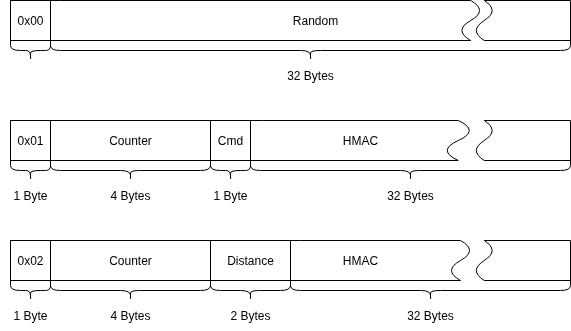
\includegraphics[height=50mm]{images/MessageLayout.png}
	\centering
	\caption{Layout of Messages}
	\label{fig:msg}
\end{figure}

\section{Program flowchart}
\label{chapter3}


\paragraph{}
\ref{fig:stateDiagrams} shows the state transition diagrams for Node 1 and Node 2. Both nodes execute a thread that sets up the Bluetooth communication and sends and receives data. Node 1 executes a second thread which periodically fetches the proximity sensor readings, and provides them to the communication thread for transmission to Node 2. Node 2 executes a thread which uses the current speed and distance data to automatically control the vehicle speed if the ACC system is turned on.

\begin{figure}[h]
	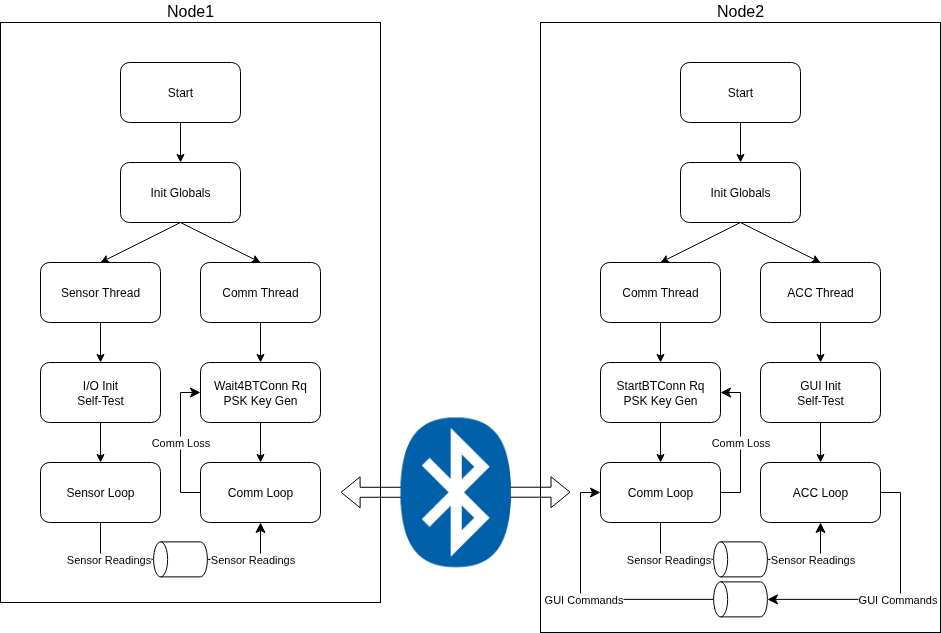
\includegraphics[height=100mm]{images/StateDiagrams.png}
	\centering
	\caption{State Diagrams}
	\label{fig:stateDiagrams}
\end{figure}

\paragraph{}
\ref{fig:stateDiagramNode1} shows the two thread loops of Node 1 in more detail. The Sensor Loop sequentially obtains readings from the two connected sensors, checks the value for plausibility and consistency. Depending on whether values are OK, the thread pushes the normalized distance data or an error code to a global variable, where the communication thread picks it up for further transmission. In the end, the thread is put to sleep for a short amount of time after which it starts over.

\paragraph{}
The communication loop waits for request messages to be received. If an error happens during data reception, the Bluetooth connection is closed and a new one is set up. On successful message reception, the data is parsed and checked for authenticity and validity (i.e. the MAC and counter values are verified for correctness). Requests which fail these checks are ignored. If the received message turns out to be a request for a transmission of the distance readings, the thread picks up the distance data from a global variable and puts it into a message which it transmits to Node 2. If the transmission fails, the Bluetooth transmission is closed again and a new one is set up. On successful transmission, the thread puts itself to sleep for a short amount of time after which it starts over.

\paragraph{}
The steps in diagram \ref{fig:stateDiagramNode1} which are drawn in inverted color involve read or write operations on shared global data. In order to avoid race conditions the read/write operations are protected in critical sections.

\begin{figure}[h]
	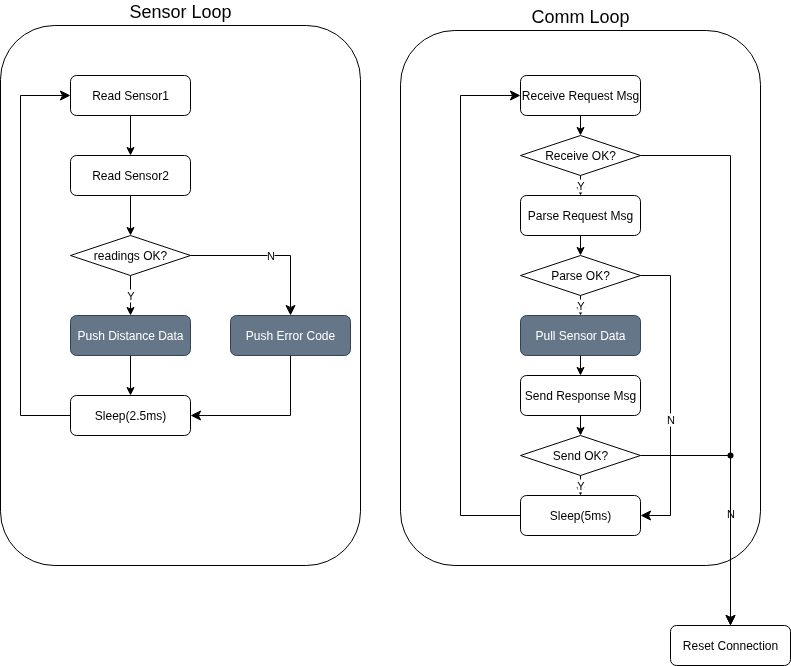
\includegraphics[height=100mm]{images/StateDiagramNode1.png}
	\centering
	\caption{State Diagrams Node 1}
	\label{fig:stateDiagramNode1}
\end{figure}

\paragraph{}
\ref{fig:stateDiagramNode2} shows the two thread loops that execute on Node 2. The communication loop sends a request message for a new distance reading value to Node 1. If the response message passes the authenticity and validity checks, the received sensor data is copied into a global variable where it can be picked up from the ACC thread. In the last step the thread puts itself to sleep for a short amount of time, after which it starts over. Similar to Node 1, if either message reception or transmission fails, the current connection is closed and a new one is set up. Received messages which fail authenticity and validity checks are ignored.

\paragraph{}
The ACC loop retrieves from the GUI the ACC status (whether the driver has turned it on or off) and, if it is turned off, the current, manually set, speed. In the next step, it obtains the Sensor data (i.e. the most recently received distance data). It verifies whether an error code or a valid distance was received, and also whether the age counter of the reading lies within the allowed threshold. If either age or value indicate an error, an error counter is incremented. If the error counter is above a given threshold of four incorrect readings, the state of the ACC is set to ERROR. If the error counter lies below that threshold the distance reading is ignored (and the last successful distance is used in the subsequent steps instead). If both value and age of the reading are OK, the reading is accepted as current distance, moreover the state of the ACC is set to OFF if it was previously in the ERROR state.
In the next step, if ACC is in the ON state, a control function \emph{Speed = ACC(Distance, Speed)} is applied, i.e. the ACC accelerates/decelerates the car depending on the current vehicle speed and measured distance.
Thereafter, the current vehicle speed, distance, and ACC state is conveyed to the display so it can update the corresponding GUI elements. In the last step, the control loop puts itself to sleep for a short amount of time and thereafter starts over. Like in the previous diagram, steps in inverted color indicate read/write accesses to data shared across threads. These accesses are protcted by critical sections.

\begin{figure}[h]
	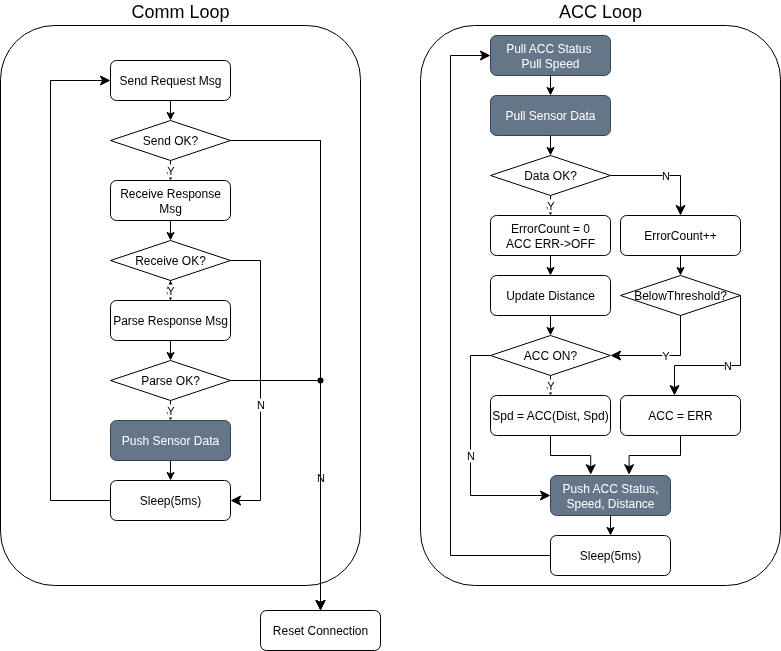
\includegraphics[height=100mm]{images/StateDiagramNode2.png}
	\centering
	\caption{State Diagrams Node 2}
	\label{fig:stateDiagramNode2}
\end{figure}

\section{Hazard identification}
\label{chapter4}

This chapter focuses on hazards. The emphasis is on preventing injury to living beings while ensuring the best possible use of the ACC.

\subsection{Identified hazards and countermeasures}


	\begin{enumerate}
		\item \textbf{Hazard 1:} Sensor failure - incorrect distance measurement
            
            \textbf{Description:} A failure or malfunction of an ultrasonic sensor can lead to implausible distance values. This can result in obstacles not being detected or incorrect distances being transmitted. Since speed control depends directly on these measured values, this poses a significant safety risk.
            
            \textbf{Solution:} Use of two redundant sensors.
%			Requirement see \ref{req.1.1} \\

        \paragraph{}
		\item \textbf{Hazard 2:} Bluetooth Connection Loss
            
            \textbf{Description:} A connection failure between Node 1 and Node 2 via the Bluetooth interface means that distance information can no longer be transmitted. As a result, Node 2 loses the basis for speed control, which can lead to unsafe driving behavior.
            
            \textbf{Solution:} Implementation of a timeout mechanism: If no valid data is received within, for example, 500 ms, the ACC system is automatically deactivated. + Alarm indicator on the display to alert the driver to the failure.
%			Requirement see \ref{req.1.1} \\
        
        \paragraph{}
		\item \textbf{Hazard 3:} Sensor inconsistency
            
            \textbf{Description:} Even if both sensors are still working, their measured values may differ from each other (e.g., due to interference, different reflection angles, or partial coverage). This inconsistency can lead to incorrect decisions in speed control.
            
            \textbf{Solution:} Consistency check: The measured values of both sensors are compared with each other. If the difference exceeds a defined threshold value, the result is considered inconsistent.
%			Requirement see \ref{req.1.1} \\
        
        \paragraph{}
	\end{enumerate}
	
\subsection{Identified hazards without countermeasures }

	\begin{enumerate}
		\item \textbf{Hazard 1:} Electric shock

            \textbf{Description:} Exposed cables may cause electric shocks if touched. This hazard is not taken into account as we are dealing with a prototype.
            
        \paragraph{}
		\item \textbf{Hazard 2:} Environmental factors that affect sensor accuracy (Humidity, Temp. e.g.)
        
            \textbf{Description:} This would require a laboratory environment; instead, we cover redundancies.

        \paragraph{}
		\item \textbf{Hazard 3:} Power failure
        
            \textbf{Description:} We recognize power failure as a hazard, but we assume that we have a reliable power supply.


	\end{enumerate} 
\section{Threat identification}
\label{chapter5}

\subsection{Identified threats and countermeasures}


	\begin{enumerate}
		\item \textbf{Threat 1:} Manipulation during Transmission (Tampering)
            
            \textbf{Description:} An attacker could attempt to alter the messages transmitted between Node 1 and Node 2. This could result in false sensor data or control commands being introduced, leading to dangerous situations (e.g., incorrect distance = incorrect speed control). The point at which the problem occurs can be seen in Figure \ref{fig:stateDiagrams} at the Bluetooth symbol.
            
            \textbf{Solution:} Data integrity is ensured by an HMAC (hash-based message authentication code). The solution process can be seen in Figure \ref{fig:stateDiagramNode1} in the “Send Sensor Msg”-block of the Comm Loop.
%			Requirement see \ref{req.1.1} \\
        
        \paragraph{} 
		\item \textbf{Threat 2:} Denial of Service (DoS)
            
            \textbf{Description:} An attacker or jammer could block the Bluetooth connection (e.g., through jamming or flooding). This would render sensor data unavailable and cause the ACC to lose its basis. The point at which the problem occurs can be seen in Figure \ref{fig:stateDiagrams} at the Bluetooth symbol.
            
            \textbf{Solution:} Implementation of a timeout mechanism for Bluetooth messages. If the connection fails for longer than a defined period of time, the system automatically switches to manual operation. The solution process can be seen in Figure \ref{fig:stateDiagramNode2} in the “Receive Ok?” block of the Comm Loop.
%			Requirement see \ref{req.1.1} \\
        
        \paragraph{} 
		\item \textbf{Threat 3:} Replay-Attack (Spoofing)
            
            \textbf{Description:} An attacker could resend previously intercepted messages to Node 2 (replay). This could allow outdated but formally valid distance data to be used, leading to dangerous rule decisions. The point at which the problem occurs can be seen in Figure \ref{fig:stateDiagramNode2} at the "Receive Sensor Msg (Blocking)"-Block of the Comm Loop.
            
            \textbf{Solution:} Use of a sequence counter or sequential message number in each packet.
%			Requirement see \ref{req.1.1} \\
        
        \paragraph{} 
	\end{enumerate}
	
\subsection{Identified threats without countermeasures}

\begin{enumerate}
		\item \textbf{Threat 1:} Preshared Key not protected (Spoofing)

            \textbf{Description:} The preshared key is stored openly in the repository. If accessed by unauthorized persons, it could be used to impersonate trusted nodes. This is acceptable for the prototype stage, but proper key storage should be implemented in production. The point at which the problem occurs can be seen in Figure \ref{fig:stateDiagramNode2} at the "Receive Sensor Msg"-Block of the Comm Loop.
            
        \paragraph{}
		\item \textbf{Threat 2:} No protection against buffer overflows (Denial of Service)
        
            \textbf{Description:} The code does not include checks to prevent buffer overflows. This could allow memory corruption or program crashes. As the focus lies on functionality, no memory-protection mechanisms are applied. The point at which the problem occurs can be seen in Figure \ref{fig:stateDiagramNode2} at the "Update Distance Update Timestamp ACC = OK"-Block of the ACC Loop.

        \paragraph{}
		\item \textbf{Threat 3:} Tampering on the device (Tampering)
        
            \textbf{Description:} The case where an attacker compromises the operating system of the hosts and sends forged messages on behalf of the other node is not considered. The point at which the problem occurs can be seen in Figure \ref{fig:stateDiagramNode1} at the "Send Sensor Msg"-Block of the Comm Loop.


	\end{enumerate}
 
\section{Requirements}
\label{chapter6}

“System” refers only to the ACC.

\subsection{Safety related requirements}




 \begin{enumerate}[label*=\arabic*.]
 	\item \label{req.1}  Requirement: \\
	 	The system shall be able to respond to a measurement error within 1 second by deactivating itself.  \\
	 	%Folge Requirements: \ref{req.1.1} , \ref{req.1.2}  
	 	%\begin{enumerate}[label*=\arabic*.]
	 		%\item \label{req.1.1}  Requirement  \\
	 		%At program start the LED indicating an error must be tested.\ref{req.2}\\ 
	 		%\item \label{req.1.2} Requirement   \\
	 		%At program start the USART sending error messages must be tested.\\ 
	 	%\end{enumerate}

        \item \label{req.2} Requirement: \\
        The system shall automatically detect sensor failure by checking the measured values for plausibility.  \\
	 	\item \label{req.3} Requirement: \\
        The system shall inform the driver of a detected sensor failure by means of a red LED indicator on the display. \\
        \item \label{req.4} Requirement: \\
        The system shall switch off when a sensor failure is detected. \\
        \item \label{req.5} Requirement: \\
        The system shall automatically detect a failure of the communication subsystem (Bluetooth) by recognizing that a packet could not be sent, or by recognizing that no response is received within a defined period (500 ms) after a successful transmission. \\
        \item \label{req.6} Requirement: \\
        The system is designed to inform the driver of a detected communication subsystem failure by switching on a red warning LED. \\
        \item \label{req.7} Requirement: \\
        The system shall automatically switch off when a communication subsystem (Bluetooth) error is detected. \\
        \item \label{req.8} Requirement: \\
        If a failure of the communication subsystem (Bluetooth) is detected, the system shall initiate a connection. \\
        \item \label{req.9} Requirement: \\
        The system shall inform the driver about the status of the system via a green status LED and the ACC push button display (ACC ON/ACC OFF). \\
        \item \label{req.10} Requirement: \\
        The system shall not be activated if the sensors or communication have failed. \\
        \item \label{req.11} Requirement: \\
        Once activated, the system shall note the current speed of the vehicle and not exceed it. \\
        \item \label{req.12} Requirement: \\
        The system shall deactivate when the vehicle speed falls below 30 km/h. \\
        \item \label{req.13} Requirement: \\
        The system shall reduce the speed to n/2 km/h at a measured distance of n meters. \\
	 \end{enumerate}

%Das System soll innerhalb 1 sek auf einen Fehler in der Messung reagieren können indem es sich deaktiviert.

%Das System soll einen Ausfall der Sensoren selbstständig erkennen indem es die Messwerte auf Plausibilität überprüft.

%Das System soll bei einem erkannten Sensorausfall den Fahrer durch eine Rote LED-Anzeige am Display informieren.

%Das System soll sich bei einem erkannten Sensorausfall ausschalten.

%Das System soll einen Ausfall des Kommunikationssubsystems (Bluetooth) automatisch erkennen indem es erkennt, dass ein Paket nicht versandt werden konnte, oder indem es erkennt das nach einem erfolgreichen Senden keine Antwort innerhalb eines definierten Zeitraums (10ms) bekommt.

%Das System soll bei einem erkannten Kommunikationssubsystemausfall den Fahrer durch das einschalten einer Roten Warn-LED informieren.

%Das System soll sich bei einem erkannten Kommunikationssubsystems (Bluetooth) -Fehler automatisch ausschalten.

%Bei einem erkannten Ausfall des Kommunikationssubsystems (Bluetooth) soll das System einen Verbindungsaufbau starten.

%Das System soll den Fahrer über den Zustand des Systems informieren durch eine Grüne Status-LED und durch die ACC Push Button darstellung (ACC ON/ACC OFF).

%Das System soll sich nicht Aktivieren lassen wenn die Sensoren oder die Kommunikation ausgefallen sind.

%Das System soll sobald es aktiviert wird, die derzeitige geschwindigkeit des Fahrzeugs merken und nicht überschreiten.

%Das System soll sich bei einer Unterschreitung der Fahrzeuggeschwindigkeit von 30 km/h deaktivieren.

%Das System soll bei einem gemessenen Abstand von n Metern, die Geschwindigkeit auf n/2 km/h runterregeln.




        
	 	

\subsection{Security related requirements}


\subsection{Requirements with no influence on Safety and Security}

\begin{enumerate}[label*=\arabic*.]
 	\item \label{req.1}  Requirement: \\
	 	The ACC display shall have a black background.  \\
	 	%Folge Requirements: \ref{req.1.1} , \ref{req.1.2}  
	 	%\begin{enumerate}[label*=\arabic*.]
	 		%\item \label{req.1.1}  Requirement  \\
	 		%At program start the LED indicating an error must be tested.\ref{req.2}\\ 
	 		%\item \label{req.1.2} Requirement   \\
	 		%At program start the USART sending error messages must be tested.\\ 
	 	%\end{enumerate}

        \item \label{req.2} Requirement: \\
        The speed shall be displayed in km/h.  \\
	 	\item \label{req.3} Requirement: \\
        The distance to the vehicle in front shall be displayed in meters. \\
        \item \label{req.4} Requirement: \\
        The speed shall be displayed as an integer value without decimal places. \\
        %The ESC key shall close the GUI window. \\
        \item \label{req.5} Requirement: \\
        There shall be one button for acceleration and one for deceleration in the GUI. \\
        \item \label{req.6} Requirement: \\
        The GUI shall allow the speed to be continuously increased or decreased by holding down the acceleration and deceleration buttons without the user having to tap repeatedly. \\

        
	 \end{enumerate}

 



\end{document}

